\documentclass[a4paper]{llncs}

\usepackage{amssymb}
\setcounter{tocdepth}{3}
\usepackage{graphicx}

\usepackage{url}
\urldef{\mailsa}\path|{v.bajpai, j.schoenwaelder}@jacobs-university.de|
\newcommand{\keywords}[1]{\par\addvspace\baselineskip
\noindent\keywordname\enspace\ignorespaces#1}

% added by Vaibhav
%----------------------------------------------------------------------
\usepackage[utf8]{inputenc}
\usepackage[T1]{fontenc}
\usepackage[nolist]{acronym}
\renewcommand{\ttdefault}{cmtt}

% temporaries
\usepackage{scrtime}
\usepackage{prelim2e}
\usepackage{todonotes}
\renewcommand{\PrelimWords}{\relax}
\renewcommand{\PrelimText}{\footnotesize[\,\today\ at \thistime\,]}
%----------------------------------------------------------------------


\begin{acronym}
  %\acro{NFQL}{Network Flow Query Language}
\end{acronym}

\begin{document}

\mainmatter  % start of an individual contribution

% first the title is needed
\title{From Global Measurements to Local Management}

\author{Vaibhav Bajpai \and Jürgen Schönwälder%
\thanks{This work was supported by the European Community’s Seventh Framework
Programme (FP7/2007-2013) grant no. 317647 (Leone)}}
\institute{Computer Science, Jacobs University Bremen, Germany\\
\mailsa}
\maketitle

\begin{abstract}
The abstract should summarize the contents of the paper and should
contain at least 70 and at most 150 words. It should be written using the
\emph{abstract} environment.
\keywords{Measurements, Management, IPv6}
\end{abstract}


% sections
%----------------------------------------------------------------------
\section{Introduction}
\input{sections/introduction}\label{sec:introduction}
\section{Related Work}
An interest to understand the evolution of the Internet from the user' vantage
point started with establishing techniques to remotely probe the broadband
links. Dischinger \emph{et al.} in \cite{dischinger:2007} for instance, inject
packet trains and use the responses received from gateway to infer the
broadband link characteristics. This led to development of a number of
software-based solutions, \texttt{netalyzr} \cite{kreibich:2010}, for
instance, that requires explicit interactions with the broadband consumer.
Recently, the requirement for accurate measurements, coupled with \ac{FCC}'
initiated efforts to define data-driven standards has led to the deployment of
a number of large-scale measurement platforms that perform measurements using
dedicated hardware probes not only from within the ISP' network but also
directly from the home gateway.

% samknows and bismark
SamKnows \footnote{\url{http://www.samknows.com}} specializes in such
measurements to study the performance of broadband access networks. It
functions by deploying dedicated hardware probes in the home gateway, that
perform active measurements when the user is less aggresively using the
network. In a recent study, sponsered by the \ac{FCC}, Sundaresan \emph{et
al.} \cite{sundaresan:2011} have used this measurement data to investigate the
throughput and latency of access network links across multiple ISP's. in the
United States. They have coupled this data with their own Bismark platform
\cite{sundaresan:2012} to investigate different traffic shaping policies
enforced by the ISP and understand the bufferbloat phenomenon
\cite{gettys:2012}. The empirical findings of this study has recently been
repraised by Canadi \emph{et al.} in \cite{canadi:2012} where they use
crowdsourced data from \url{speedtest.net} to compare both results.

% ripe atlas
Ripe Atlas \footnote{\url{https://atlas.ripe.net}} is another independent
measurement infrastructure deployed by \ac{RIPE NCC}. It consists of thousands
of probes distributed around the globe that perform \ac{RTT} and traceroute
measurements to a number of preconfigured destinations alongside DNS queries
to root DNS servers.

% measurement lab
\ac{M-Lab} \cite{dovrolis:2010} is an open, distributed platform to deploy
internet measurement tools and the resulting measurement data on Google'
storage infrastructure. The tools vary from measuring TCP throughput and
available bandwidth to emulating clients to identify end-user traffic
differentiation policies \cite{dischinger:2010, kanuparthy:2011} to performing
reverse traceroute lookups from arbitrary destinations \cite{bassett:2010}.
All of the collected data is available in the public domain.
\label{sec:relatedwork}
\section{Preliminary Results}
\begin{figure}[t]
  \begin{minipage}[t]{0.50\textwidth}
    \centering
    \resizebox*{1.0\textwidth}{!}{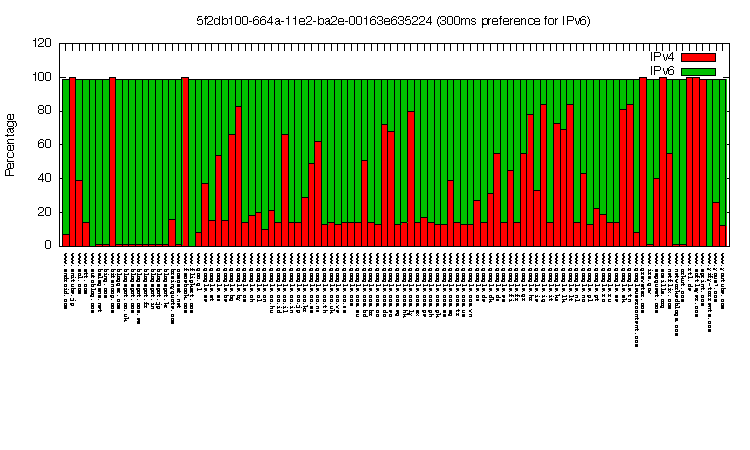
\includegraphics{figures/t28971-competition-300ms}}
    \caption{Native IPv4 and Teredo Tunnel}
  \end{minipage}
  \begin{minipage}[t]{0.50\textwidth}
    \centering
    \resizebox*{1.0\textwidth}{!}{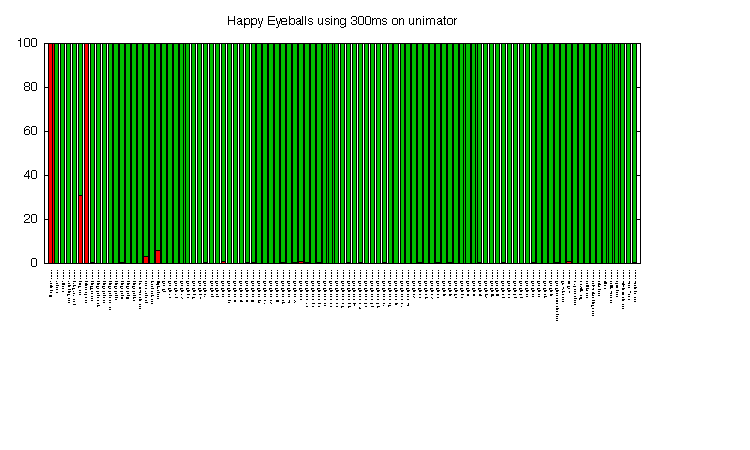
\includegraphics{figures/unimator2-competition-300ms}}
    \caption{Native IPv4 and Native IPv6}
  \end{minipage}
\caption{\label{fig:happy-v4-v6-compete}IPv4 and IPv6 Happy Eyeball Competition} 
\end{figure}

A user when attempting to connect to a dual-stacked web service prefers
connecting over IPv6. This is because in POSIX systems, the domain name
resolution system call \texttt{getaddrinfo(\ldots)} returns a list of
endpoints in an order that prioritizes an IPv6-upgrade path \cite{rfc6724}.
The dictated order can dramatically reduce the application responsiveness in
situations where IPv6 connectivity is broken. This is because, the attempt to
connect over an IPv4 endpoint will take place only when the IPv6 connection
attempt has timed out, which can be in the order of seconds.

\begin{figure}[t]
  \begin{minipage}[t]{0.50\textwidth}
    \centering
    \resizebox*{1.0\textwidth}{!}{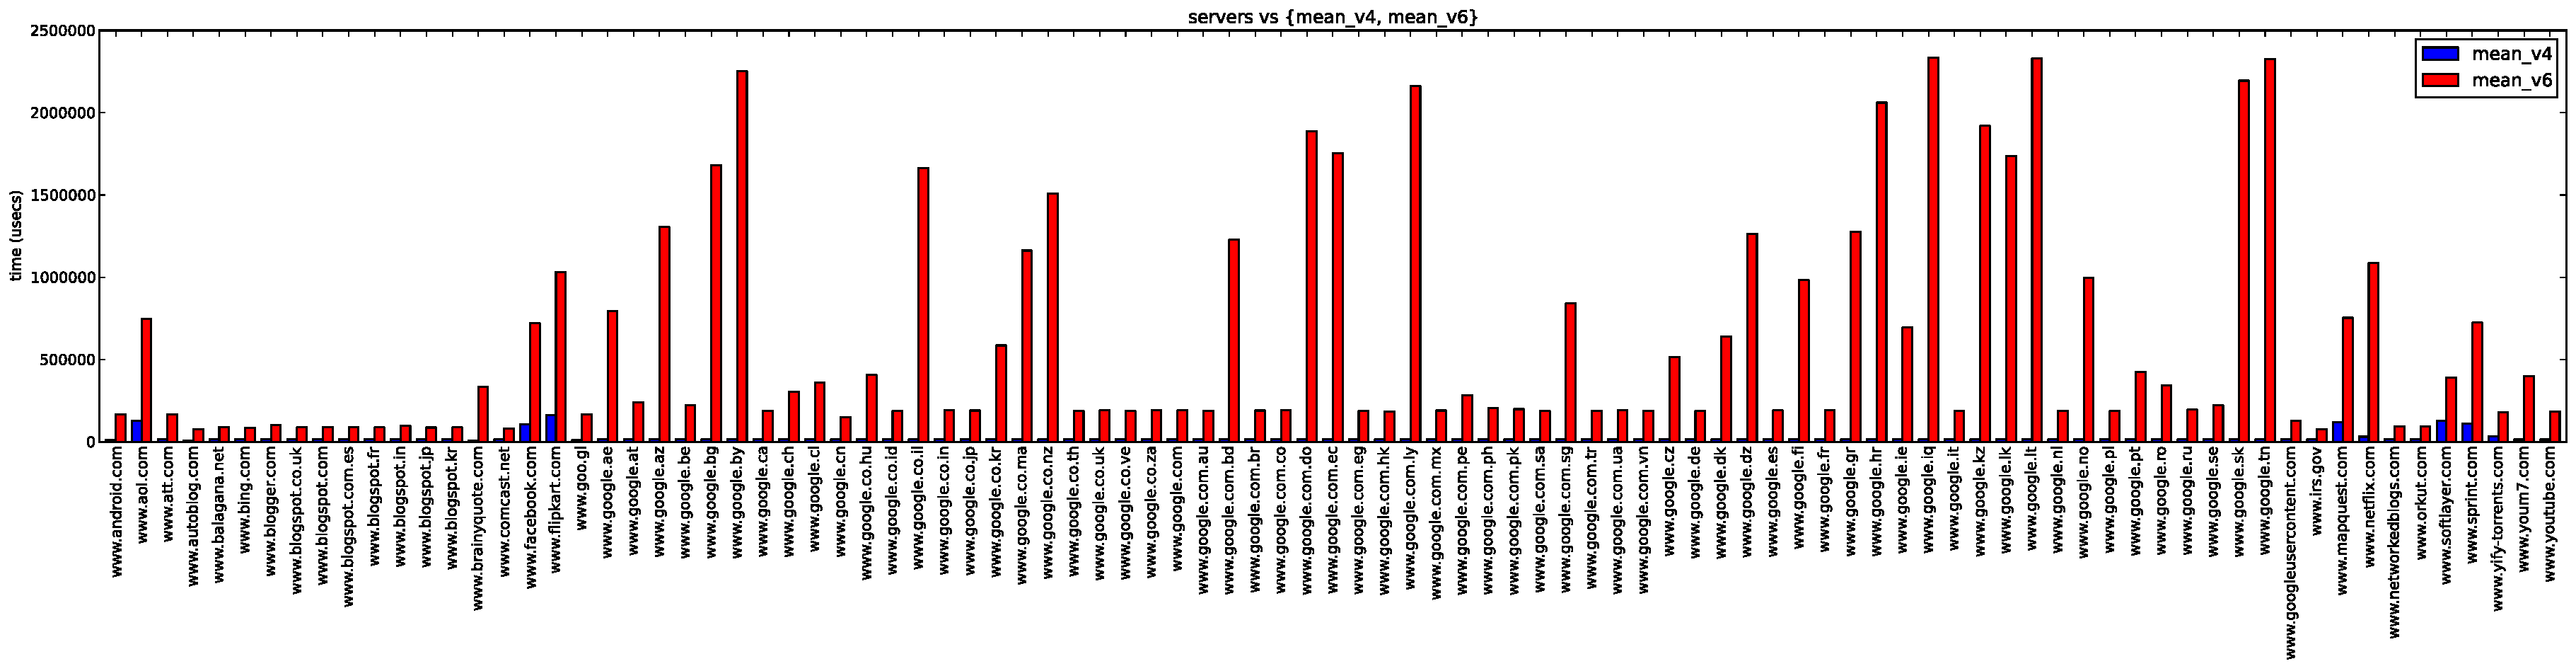
\includegraphics{figures/t28971-mean}}
    \caption{Native IPv4 and Teredo Tunnel}
  \end{minipage}
  \begin{minipage}[t]{0.50\textwidth}
    \centering
    \resizebox*{1.0\textwidth}{!}{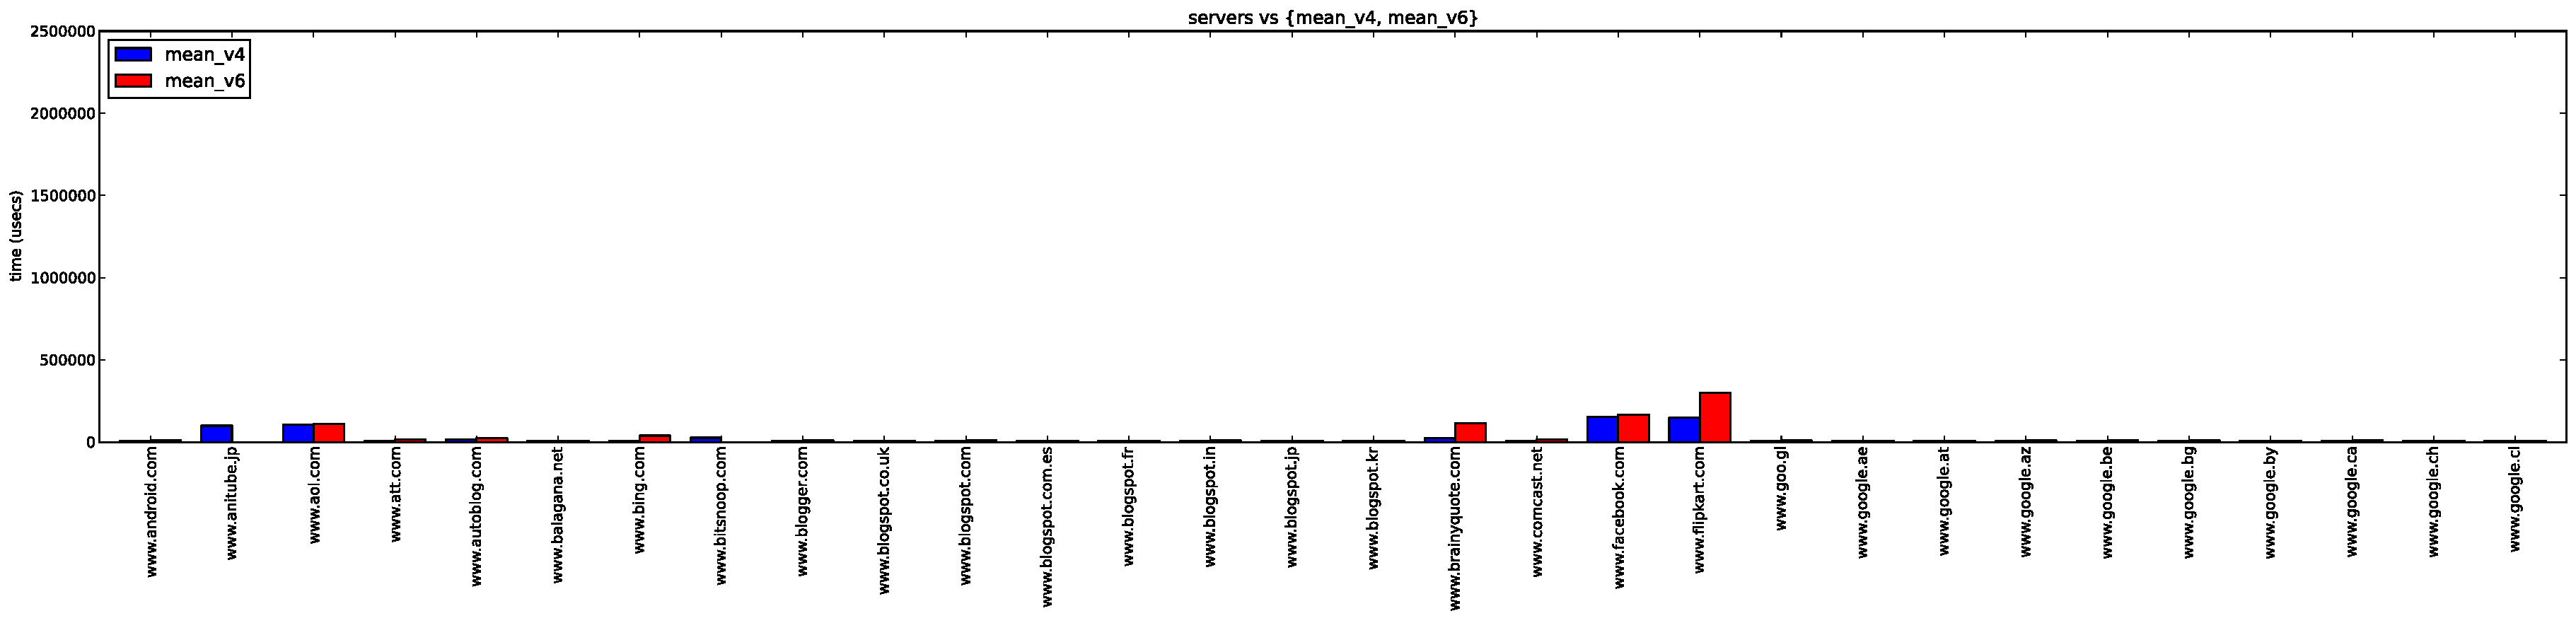
\includegraphics{figures/unimator2-mean}}
    \caption{Native IPv4 and Native IPv6}
  \end{minipage}
\caption{\label{fig:happy-v4-v6-mean-std} Mean and Standard Deviations for
IPv4 and IPv6}
\end{figure}

This noticeable degraded user experience can be subverted by making
applications apply the happy eyeballs algorithm \cite{rfc6555}. The algorithm
recommends that a dual-stacked application resolves the DNS names of a
dual-stacked service for both IPv4 and IPv6 endpoints at once. If the resolver
returns both endpoints, the application must try a TCP
\texttt{connect(\ldots)} to both the endpoints pick the one that
completes first. The connection attempt does prefer the first resolved
address family (usually IPv6) by the order of 300ms though.

In this pursuit, to determine whether applications will use IPv4 or IPv6 on a
dual stacked service, we developed \texttt{happy}, a simple TCP happy eyeballs
probing tool. It uses non-blocking \texttt{connect(\ldots)} calls to
concurrently establish connections to all the endpoints of a service.
%The tool, however, does not check whether the endpoints of a given target all
%provide the same service. Hence, it is possible to impact the results by
%setting up fake servers that do not provide the service tested and which are
%designed and deployed with the only purpose to provide fast connection setup
%times and redirect services.
We have cross-compiled \texttt{happy} for the
OpenWRT\footnote{\url{https://openwrt.org}} platform, so that the tool can now
be run on widely deployed SamKnows probes. In order to ascertain the value in
this approach and develop data analysis tools, we prepared an internal
test-bed of multiple measurement points. The measurement points have different
flavors of IPv4 and IPv6 connectivity ranging from native IPv4, native IPv6,
IPv6 tunnel broker endpoints, Teredo and tunnelled IPv4. We used the top 100
DNS names compiled by Hurricane Electric Internet
Services\footnote{\url{http://bgp.he.net/ipv6-progress-report.cgi}} and ran
\texttt{happy} on the set of dual-stack services represented by these DNS
names.

\begin{figure}[t]
  \begin{minipage}[t]{0.50\textwidth}
    \centering
    \resizebox*{1.0\textwidth}{!}{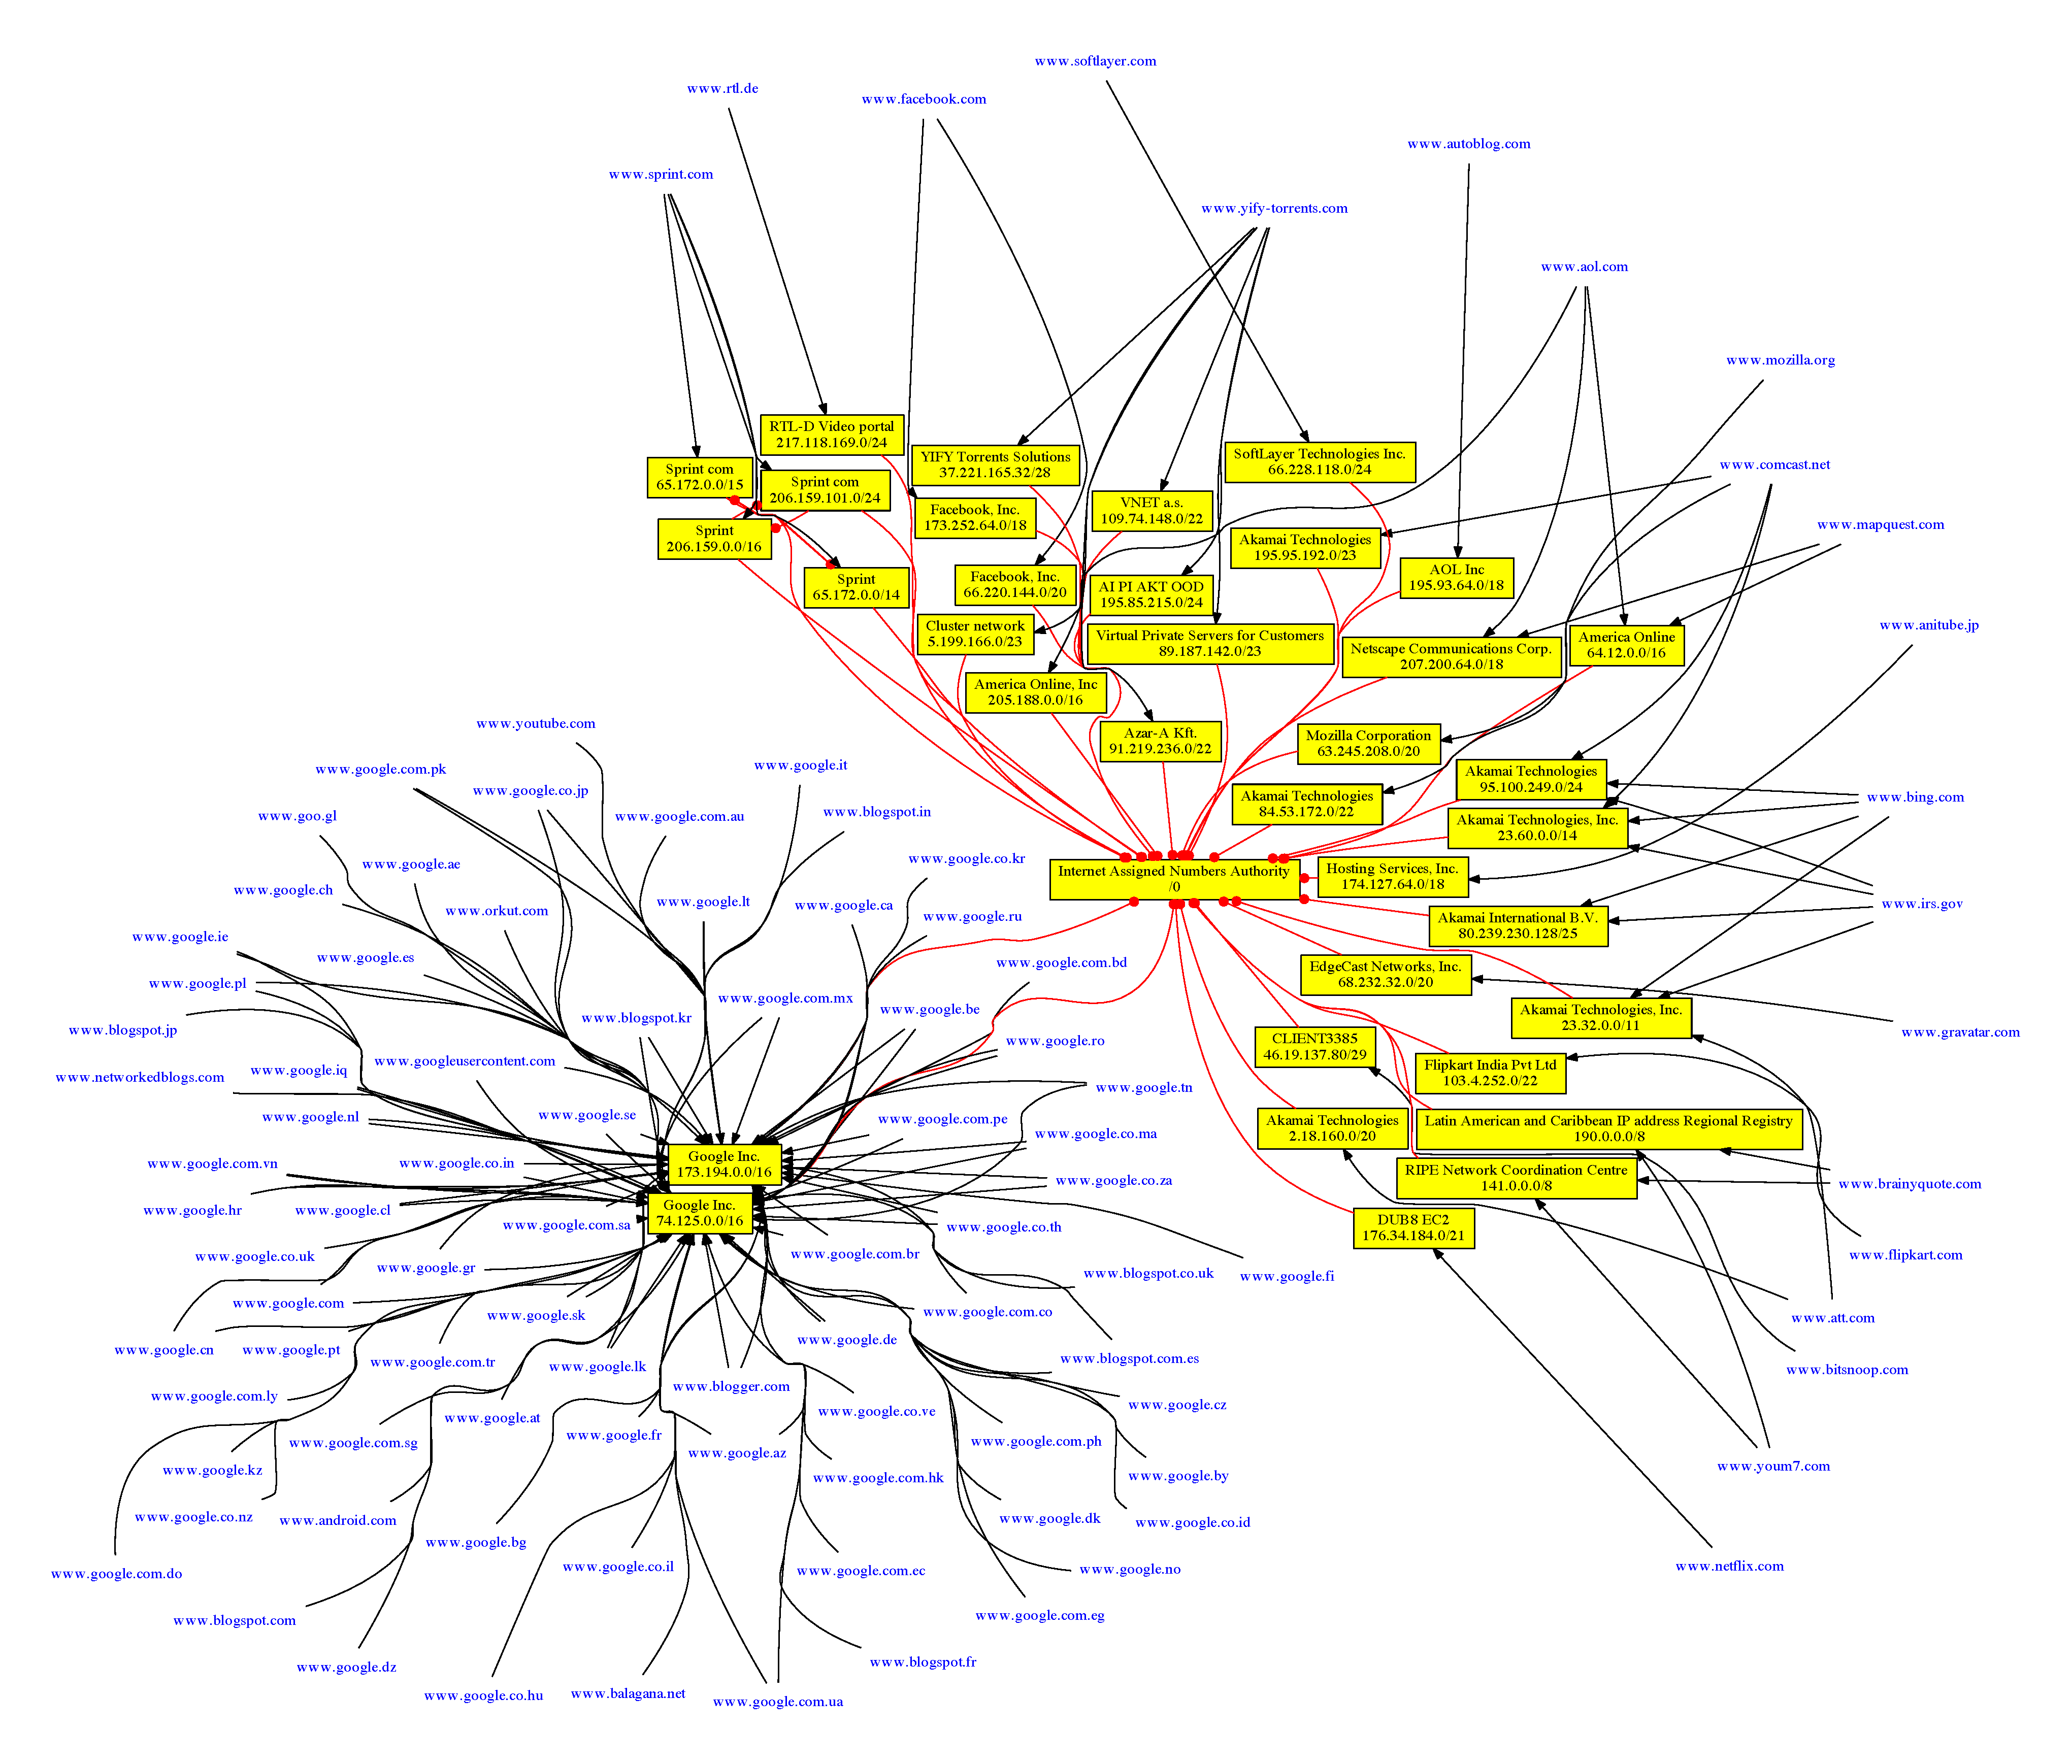
\includegraphics{figures/happy-v4cloud}}
  \end{minipage}
  \begin{minipage}[t]{0.50\textwidth}
    \centering
    \resizebox*{1.0\textwidth}{!}{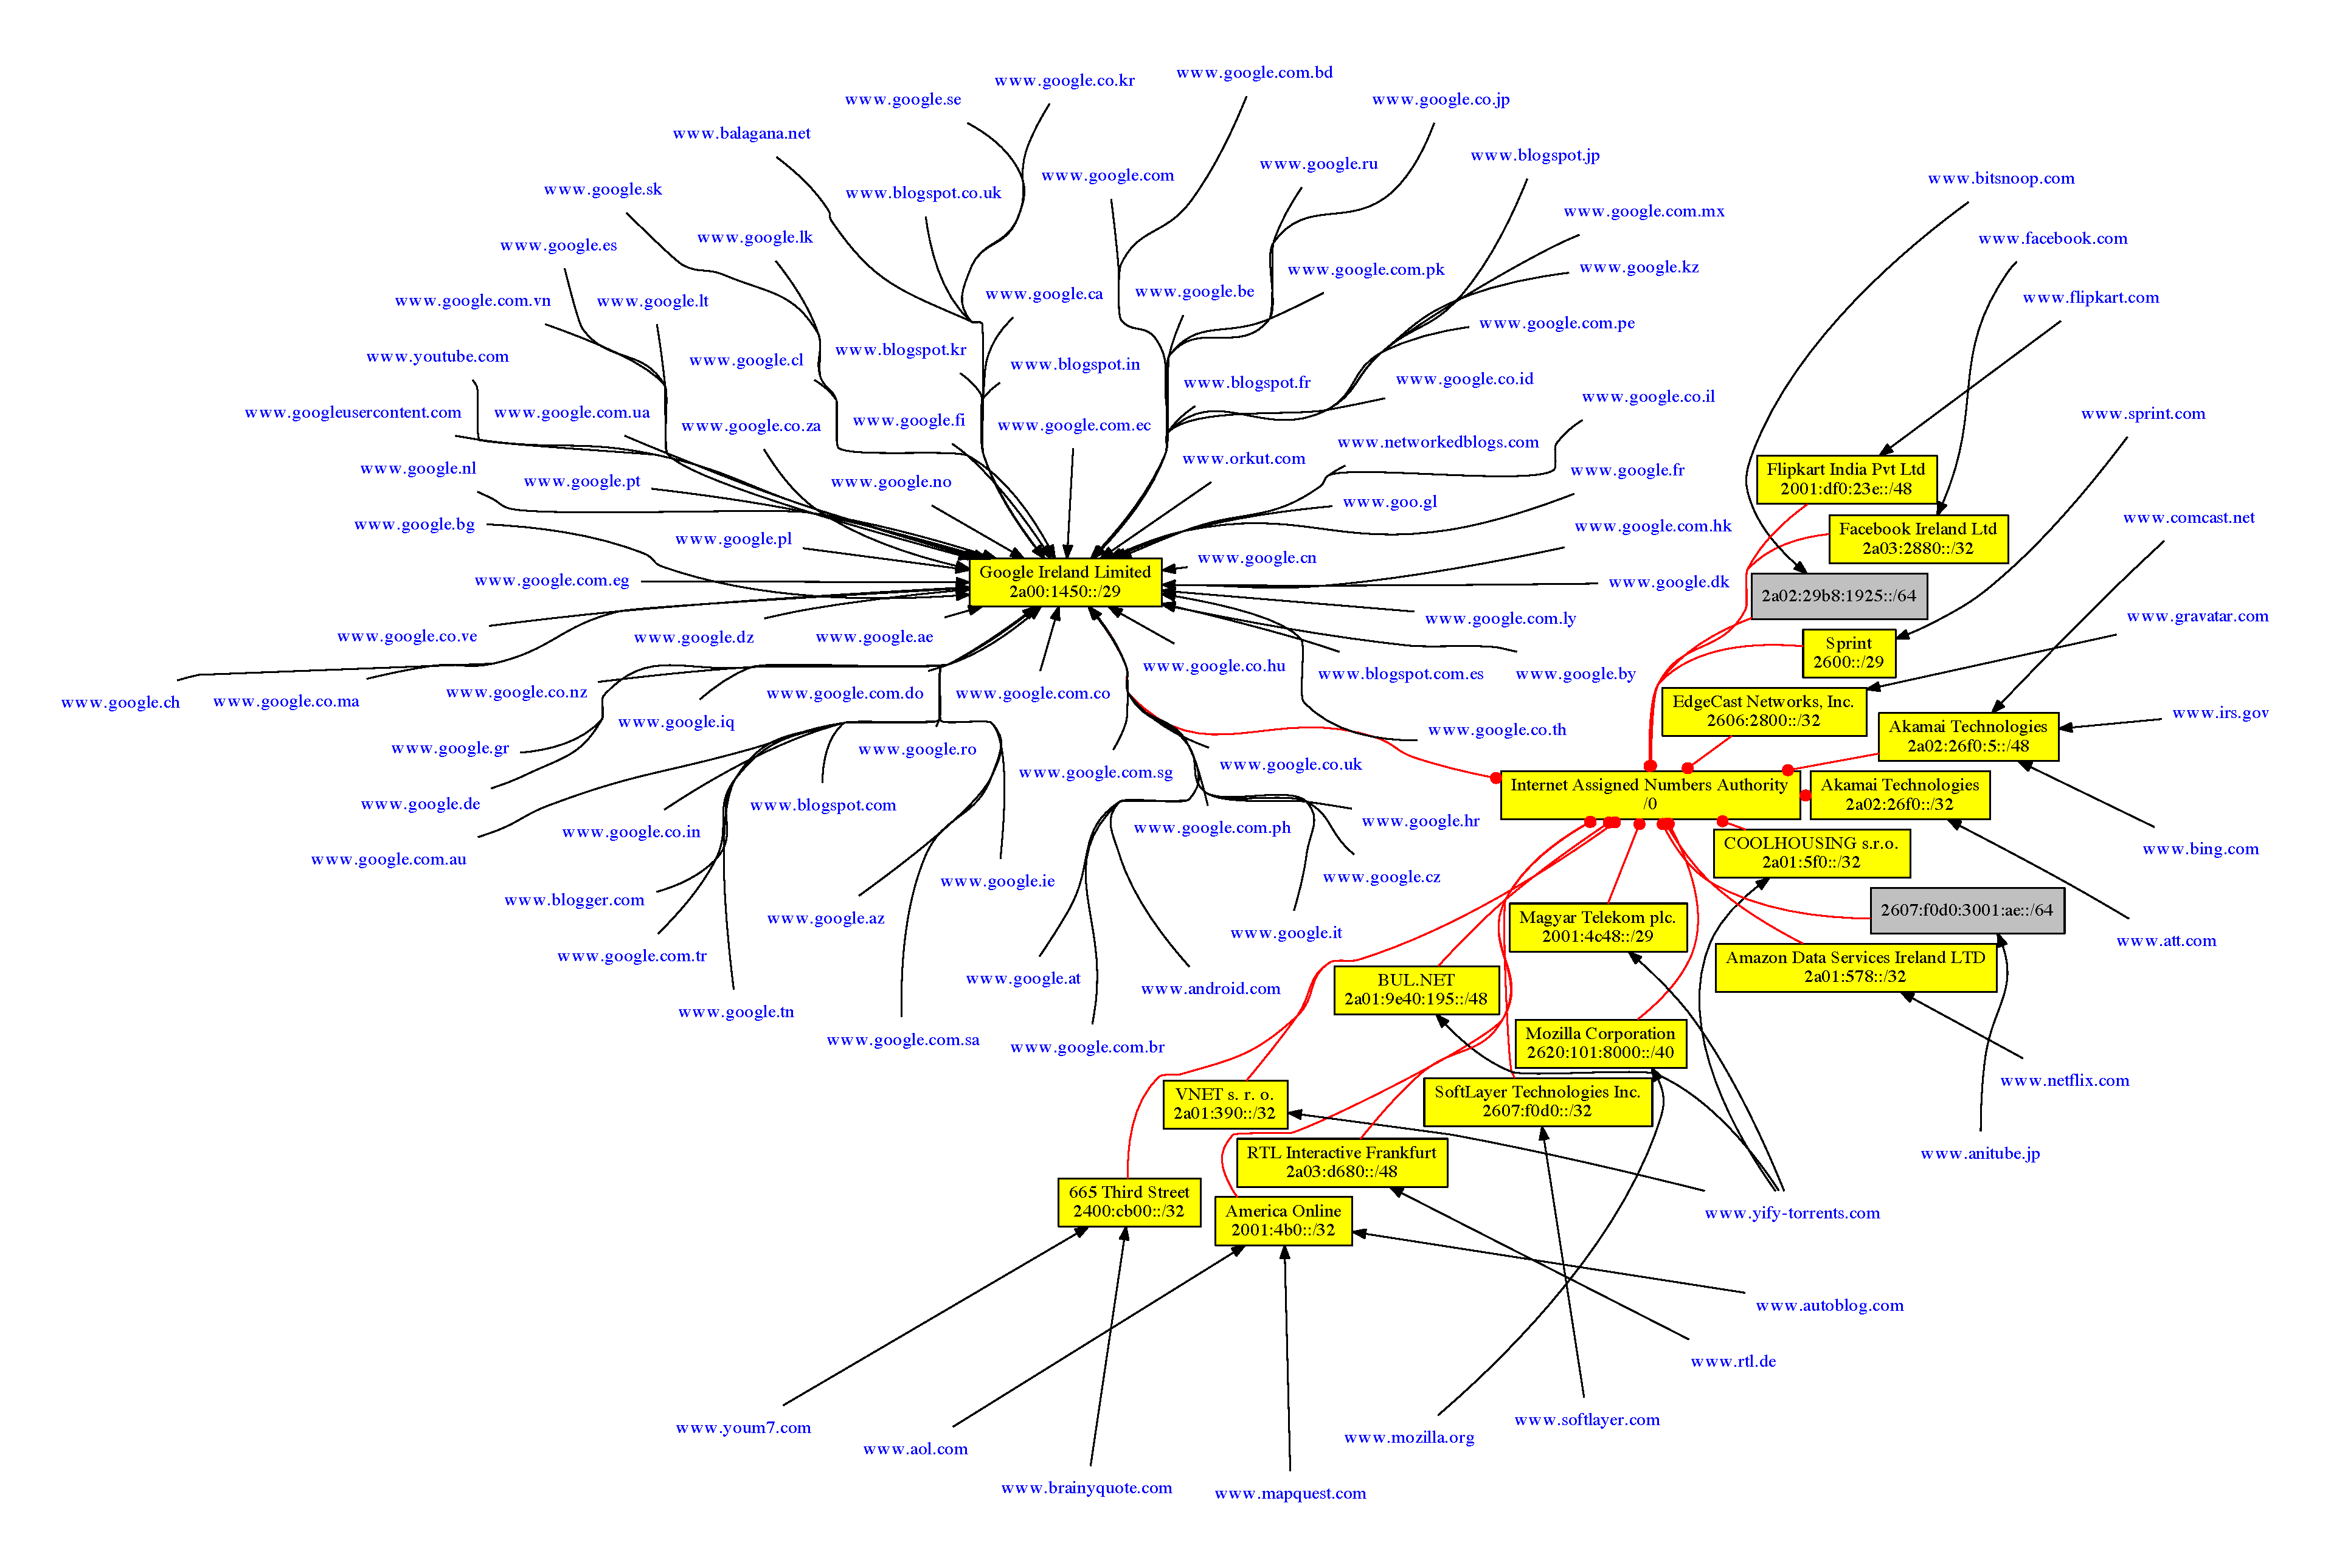
\includegraphics{figures/happy-v6cloud}}
  \end{minipage}
  \caption{\label{fig:v4-v6-cloud}An IPv4 and IPv6 aggregation cloud depicting
how most of the services centralize on core content delivery networks and
major cloud platforms}
\end{figure}

A preliminary result comparing the preference of a happy-eyeballed application
to IPv6 and IPv4 from two measurement points is shown in Fig.
\ref{fig:happy-v4-v6-compete}. The initial results show that happy eyeballs
prevents IPv6 access to Facebook, with only a 20\% chance to get to Google
related services over a Teredo Tunnel. The results look more promising on a
native IPv6 connection. It is important to note that adhering to the happy
eyeballs recommendation, IPv6 endpoints are allowed a 300ms chance to succeed.
A result comparing the time (mean and standard deviation) to establish a TCP
connection to each of the services from the same measurement points is shown
in Fig. \ref{fig:happy-v4-v6-mean-std}. The initial results show higher time
variances when connections are made over IPv6. In addition, it appears, some
of the related (and few of the unrelated) services show very similar
performances.  These services either resolve to the same endpoint or a set of
endpoints that belong to the same allocated prefix. Digging through the
\texttt{whois} information for each of the endpoints from their \ac{RIR} seems
to indicate that major portion of the services map to allocated prefixes owned
by popular organizations like Google and Akamai Technologies as shown in Fig.
\ref{fig:v4-v6-cloud}\footnote{A full resolution image is available at
  \url{https://gist.github.com/vbajpai/4730696}}

%As much as it is important to define and implement new tests on these
%measurement infrastructure, it is also equally pertinent to not only be able
%to install, update and delete these tests but also configure the entire suite
%of probes using a standardized protocol over the network. The \ac{NETCONF}
%protocol \cite{rfc6241} is particularly designed to cater to this problem.
%Towards this end, we have built a \ac{NETCONF} server for the OpenWRT platform
%using the \texttt{libnetconf}
%\footnote{\url{http://code.google.com/p/libnetconf/}} library and tested the
%implementation using our NETCONF Python API \texttt{ncclient}
%\cite{sbhushan:2009}. This will allow automated deployment of measurement
%tests and remote management of their startup configurations.

\label{sec:preliminaryresults}
\section{Future Work}\label{sec:futurework}
In the past, we performed an experimental evaluation of IPv6 transitioning
technologies to identify how well current applications and protocols
interoperate in such a deployement scenario \cite{vbajpai:2012}. In the
future, we want to study and compare the performance of IPv6 with respect to
IPv4 from a dual-stacked home gateway.  We are also interested to define
metrics that can identify whether the home gateway is behind a \ac{CGN}  or is
otherwise encompassed by several layers of \ac{NAT}s enforced by the ISP.

In our preliminary study, we have witnessed that a major portion of the
services in practicality centralize either on core content delivery networks
or major cloud platforms. We want to investigate this effect in more detail
and understand to what extend does this network aggregation and the eventual
user experience depend on the localization information.

Our current NETCONF server implementation for the SamKnows platform assumes
the existence of an ssh server implementation that provides subsystem support.
We would like to subvert this limitation and instead secure NETCONF exchanges
over TLS \cite{draft-ietf-netconf-rfc5539bis-01}. We are also interested to
define new YANG \cite{rfc6020} data models for configuring and scheduling the
measurement tests for such large-scale broadband access measurements. These
data models can be used with either \ac{NETCONF} or using a RESTful interface
\cite{draft-bierman-netconf-yang-api-01}.

\section{Conclusion}
We have performed a preliminary study on how IPv6 deployment may affect the
\ac{QoE} of Internet users. Using a large-scale measurement platform we want
to take this further, and define new metrics, measurement tests and data
analysis tools that help us understand the impact of network infrastructure
changes.
\label{sec:conclusion}
%----------------------------------------------------------------------



% bibliography
%----------------------------------------------------------------------
\bibliographystyle{splncs}
\bibliography{index}
%----------------------------------------------------------------------

\end{document}
